\newpage
\section{Dual-Slope Verfahren}
Der Dual-Slope-Umsetzer integriert zuerst die Eingangsspannung \(U_e\) während einer festen Zeit \(t_1\), wobei die Integratorspannung linear ansteigt. Nach \(t_1\) wird auf eine konstante Referenzspannung \(U_{\text{ref}}\) mit umgekehrtem Vorzeichen umgeschaltet. Der Integrator läuft wieder auf 0 zurück. Während dieser Rückintegration zählt ein Zähler die Taktimpulse über die Zeit \(t_2\) bis zum Nulldurchgang, und dieser Zählerstand ist direkt proportional zur gemittelten Eingangsspannung. Da sowohl die Auf- als auch die Rückrampe durch denselben Integrator laufen, heben sich die Bauteilwerte \(R, C\) weitgehend heraus, und durch geeignete Wahl von \(t_1\) lassen sich z.\,B.\ Netzbrumm-Störungen (50\,Hz) gut unterdrücken.

\subsection{Aufgabenstellung}
Die Funktion des Dual{-}Slope{-}Konverters soll zunächst kurz in eigenen Worten beschrieben und das Verfahren anschließend gemäß der Skizze in \autoref{fig:40_schaltung} aufgebaut werden.

Zunächst ist der Umsetzer mit dem manuellen Starter zu überprüfen. Dabei werden auch der Integratorausgang und die Schalterstellungen der Ablaufsteuerung aufgenommen. Danach sind Integratorausgang und Taktsignal (CLK und \(n\!\cdot\!\mathrm{CLK}\)) für verschiedene Eingangsspannungen zu messen. Auf Basis dieser Messungen wird die Umsetzerkennlinie mit einem der beiden Taktsignale aufgenommen und auf Missing Codes sowie Monotonie-Fehler untersucht.
Zum Abschluss sollen am Summationsverstärker Störungen mittels Rauschquelle und sinusförmigem Signal simuliert werden. Die Auswirkungen sind im Protokoll zu beschreiben und der zeitliche Verlauf darzustellen. Eine zusätzliche Kennlinie ist nicht erforderlich.


\subsection{Aufbau}
Der Versuchsaufbau folgt der in der Abbildung dargestellten Dual-Slope-Schaltung. Die Eingangsspannung $U_e$ wird über den Eingangsverstärker auf ein geeignetes Niveau bezogen auf die interne Referenz gebracht und anschließend dem Integrator zugeführt. In der ersten Phase integriert dieser die Messspannung, während in der zweiten Phase auf die konstante Referenzspannung von \SI{-5}{\volt} umgeschaltet wird, wodurch der Integrator mit definierter Steigung zum Nullpunkt zurückläuft.

Der Komparator erkennt den Nulldurchgang und erzeugt das End-of-Conversion-Signal, wodurch die Ablaufsteuerung den Zähler stoppt. Die Anzahl der während der Rücklaufphase gezählten Taktimpulse ist proportional zur Eingangsspannung und wird über die Anzeige als digitales Messergebnis ausgegeben.


\begin{figure}[h]
	\centering
	
\includegraphics[width=0.95\textwidth]{49_dualslope_schaltplan.png}
	\caption{Schaltplan für Dual-Slope-Verfahren}\label{fig:40_schaltung}
\end{figure}


\subsection{Manueller Betrieb}
Im manuellen Modus wird der Messzyklus nicht automatisch gestartet, sondern über den Taster ausgelöst. Der Taster ersetzt das Startsignal der Ablaufsteuerung, während der Zählvorgang weiterhin vom Taktsignal (CLK bzw.\ \(n \cdot \mathrm{CLK}\)) bestimmt wird. Beim Betätigen des Tasters beginnt die Aufintegration von \(U_e\), bis auf die Referenzspannung \(U_{\text{ref}}\) umgeschaltet und die Rückintegration eingeleitet wird.

Da der Taster nicht mit konstanter zeitlicher Präzision betätigt werden kann, eignet sich der manuelle Modus nur zur Demonstration des Ablaufs, jedoch nicht zur korrekten Codebildung. Mehrere Tastendrücke sind notwendig, um den vollständigen Messzyklus auszulösen, wodurch keine reproduzierbare Umsetzung erreicht wird.

\subsection{Ausgangsspannung $U_a$ des Integrators bei Takt CLK und $n\cdot$CLK}

Die Ausgangsspannung $U_a$ des Integrators wurde zusammen mit dem Taktsignal für verschiedene Eingangsspannungen gemessen. Dazu wurden die Werte \(U_e \in \{-2\,\mathrm{V}, 0\,\mathrm{V}, 2\,\mathrm{V}\}\) eingestellt und jeweils Oszillogramme für Takt = CLK (vgl.\ Abb.~\ref{fig:ua_clk}) sowie für Takt = \(n\cdot\)CLK (vgl.\ Abb.~\ref{fig:ua_nclk}) aufgenommen.
Bei der Messung mit \(n\cdot\)CLK wurde der Integrationskondensator von \(C\) auf \(C/n\) umgeschaltet, um die Integrationscharakteristik trotz verringerter Taktfrequenz vergleichbar zu halten.

In den Bildern ist erkennbar, dass die Steigung der Integrationsrampe vom Betrag und Vorzeichen der Eingangsspannung \(U_e\) abhängt: für positive Eingangsspannung steigt \(U_a\), für negative Eingangsspannung fällt \(U_a\), während bei \(U_e = 0\) nahezu keine Rampe auftritt. Gleichzeitig beeinflusst die gewählte Taktfrequenz (CLK bzw.\ \(n\cdot\)CLK) die Dauer der Integrations- und Rücksetzphase. Bei einer Testmessung mit zu hoher Eingangsspannung bzw.\ ungeeigneter Kombination von Takt und Integrationskapazität kam es zu einer Begrenzung der Integratorspannung, wobei die Spitze der Rampe abgeschnitten wurde; diese fehlerhafte Konfiguration wurde für die Auswertung nicht weiter berücksichtigt.

\begin{figure}[h]
	\centering

	% --- Row 1 ---
	\begin{minipage}[b]{0.32\textwidth}
		\centering
		
\includegraphics[width=1\textwidth]{43_clk_-2V.JPG}
		\caption*{$U_e = \SI{-2}{\volt}$}
	\end{minipage}
	\hfill
	\begin{minipage}[b]{0.32\textwidth}
		\centering
		
\includegraphics[width=1\textwidth]{40_clk_0V.JPG}
		\caption*{$U_e = \SI{0}{\volt}$}
	\end{minipage}
	\hfill
	\begin{minipage}[b]{0.32\textwidth}
		\centering
		
\includegraphics[width=1\textwidth]{41_clk_2V.JPG}
		\caption*{$U_e = \SI{2}{\volt}$}
	\end{minipage}

	\caption{
		\centering
		Ausgangsspannung $U_a$ des Integrators bei Takt = CLK, $C=C$ \\
		CH1 = $U_a$, CH2 = $U_{s1}$  CH2 = $U_{s2}$  CH2 = $U_{s3}$
	}\label{fig:ua_clk}
\end{figure}

\begin{figure}[h]
	\begin{minipage}[b]{0.32\textwidth}
		\centering
		
\includegraphics[width=1\textwidth]{44_n.clk_C-durch-n_-2V.JPG}
		\caption*{$U_e = \SI{-2}{\volt}$}
	\end{minipage}
	\hfill
	\begin{minipage}[b]{0.32\textwidth}
		\centering
		
\includegraphics[width=1\textwidth]{46_n.clk_C-durch-n_0V.JPG}
		\caption*{$U_e = \SI{0}{\volt}$}
	\end{minipage}
	\hfill
	\begin{minipage}[b]{0.32\textwidth}
		\centering
		
\includegraphics[width=1\textwidth]{48_n.clk_C-durch-n_2V.JPG}
		\caption*{$U_e = \SI{2}{\volt}$}
	\end{minipage}

	\caption{
		\centering
		Ausgangsspannung $U_a$ des Integrators bei Takt = $n\cdot$CLK, $C=C/n$ \\
		CH1 = $U_a$, CH2 = $U_{s1}$  CH2 = $U_{s2}$  CH2 = $U_{s3}$
	}\label{fig:ua_nclk}
\end{figure}

\subsection{Umsetzerkennlinie}

\subsubsection{Erkenntnis und Ergebnisse}
Aus den Messwerten des Dual-Slope-Umsetzers ergibt sich eine insgesamt etwas gleichmäßigere Kennlinie als beim Wäge-Verfahren. Missing Codes treten nicht auf, und die Abweichungen vom idealen Verlauf bleiben über alle Codes hinweg vergleichsweise gering. Dies lässt sich sowohl in der grafischen Darstellung in
\autoref{fig:40_umsetzerkennlinie} als auch in den Messwerten der
Tabelle~\ref{tab:dual_slope_adc}
erkennen. Die Endwert- und Nullpunktfehler liegen jeweils unter \(0.5\,U_{\mathrm{LSB}}\), was auf eine stabile Referenzintegration und ein weitgehend konstantes Entladeverhalten des Kondensators hindeutet.

Auch die Nichtlinearitäten sind gering: Die größte differentielle Nichtlinearität beträgt \(0.300\,U_{\mathrm{LSB}}\), während die integrale Nichtlinearität mit \(0.229\,U_{\mathrm{LSB}}\) sehr niedrig bleibt. Diese Werte sind in Tabelle~\ref{tab:dual_slope_adc_errors}
aufgeführt und bestätigen, dass der reale Verlauf dem idealen Dual-Slope-Treppenverhalten deutlich näherkommt. Damit zeigt sich die typische Stärke des Dual-Slope-Verfahrens, Störspannungen durch zeitliche
Mittelung effektiv zu unterdrücken und eine präzise Umsetzung zu ermöglichen.


\begin{figure}[h]
	\centering
	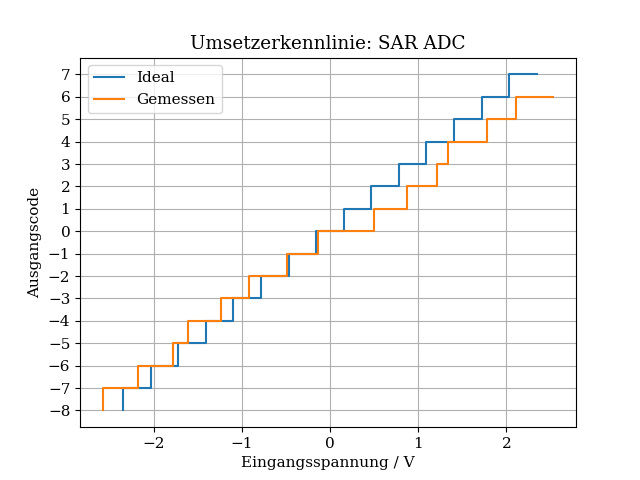
\includegraphics[width=0.7\textwidth]{images/sar_adc_curve.png}
	\caption{Umsetzerkennlinie des ADCs mit Wäge-Verfahren}\label{fig:40_umsetzerkennlinie}
\end{figure}

\begin{table}[htbp]
\centering
\caption{ADC Auswertung: Dual Slope ADC}
\label{tab:dual_slope_adc}
\begin{tabular}{c|cccc|ccc|ccc}
Code & $\dfrac{U^\mathrm{real}_{\mathrm{e}}}{\si{\volt}}$ & $\dfrac{U^\mathrm{ideal}_{\mathrm{e}}}{\si{\volt}}$ & $\dfrac{\Delta U_{\mathrm{e}}}{\si{\volt}}$ & $\dfrac{U^\mathrm{korr}_{\mathrm{e}}}{\si{\volt}}$ & $\dfrac{U^\mathrm{real}_{\mathrm{w}}}{\si{\volt}}$ & $\dfrac{U^\mathrm{ideal}_{\mathrm{w}}}{\si{\volt}}$ & $\dfrac{\Delta U_{\mathrm{w}}}{\si{\volt}}$ & $\dfrac{U^\mathrm{real}_{\mathrm{m}}}{\si{\volt}}$ & $\dfrac{U^\mathrm{ideal}_{\mathrm{m}}}{\si{\volt}}$ & $\dfrac{\Delta U_{\mathrm{m}}}{\si{\volt}}$ \\
\midrule
-8 & -2.206 & -2.344 & {\cellcolor[HTML]{35CCFF} 0.138} & -2.330 & - & - & - & - & - & - \\
-7 & -1.922 & -2.031 & 0.109 & -2.047 & 0.283 & 0.312 & 0.030 & -2.188 & -2.188 & 0.001 \\
-6 & -1.626 & -1.719 & 0.093 & -1.752 & 0.295 & 0.312 & 0.017 & -1.899 & -1.875 & 0.024 \\
-5 & -1.265 & -1.406 & 0.141 & -1.392 & 0.360 & 0.312 & 0.047 & -1.572 & -1.562 & 0.009 \\
-4 & -0.951 & -1.094 & 0.143 & -1.079 & 0.313 & 0.312 & 0.000 & -1.235 & -1.250 & 0.015 \\
-3 & -0.609 & -0.781 & 0.172 & -0.738 & 0.341 & 0.312 & 0.028 & -0.908 & -0.938 & 0.029 \\
-2 & -0.353 & -0.469 & 0.116 & -0.483 & 0.255 & 0.312 & 0.057 & -0.610 & -0.625 & 0.015 \\
-1 & -0.011 & -0.156 & 0.145 & -0.142 & 0.341 & 0.312 & 0.028 & -0.312 & -0.312 & 0.000 \\
0 & 0.293 & 0.156 & {\cellcolor[HTML]{8FFF5B} 0.137} & 0.161 & 0.303 & 0.312 & 0.010 & 0.010 & 0.000 & 0.010 \\
1 & 0.540 & 0.469 & 0.071 & 0.407 & 0.246 & 0.312 & 0.066 & 0.284 & 0.312 & 0.028 \\
2 & 0.873 & 0.781 & 0.092 & 0.739 & 0.332 & 0.312 & 0.019 & 0.573 & 0.625 & {\cellcolor[HTML]{FF728A} 0.052} \\
3 & 1.281 & 1.094 & 0.187 & 1.146 & 0.407 & 0.312 & {\cellcolor[HTML]{FFEC21} 0.095} & 0.943 & 0.938 & 0.005 \\
4 & 1.566 & 1.406 & 0.160 & 1.430 & 0.284 & 0.312 & 0.028 & 1.288 & 1.250 & 0.038 \\
5 & 1.879 & 1.719 & 0.160 & 1.742 & 0.312 & 0.312 & 0.000 & 1.586 & 1.562 & 0.024 \\
6 & 2.155 & 2.031 & {\cellcolor[HTML]{FF8438} 0.124} & 2.017 & 0.275 & 0.312 & 0.038 & 1.880 & 1.875 & 0.005 \\
7 & - & - & - & - & - & - & - & - & - & - \\
\end{tabular}
\end{table}

\begin{table}[htbp]
\centering
\caption{ADC Fehlerwerte: Dual Slope ADC}
\label{tab:dual_slope_adc_errors}
\begin{tabular}{ccccc}
Fehler & Wert in \SI{}{\volt} & Wert in $U_{LSB}$ & Wert in \% FSR & Code \\
\midrule
{\cellcolor[HTML]{FF8438} Positiver Endwertfehler} & 0.138 & 0.441 & 2.755 & -8 \\
{\cellcolor[HTML]{35CCFF} Negativer Endwertfehler} & 0.160 & 0.513 & 3.205 & 6 \\
{\cellcolor[HTML]{8FFF5B} Nullpunktfehler} & 0.137 & 0.438 & 2.735 & 0 \\
{\cellcolor[HTML]{FFEC21} Differentielle Nichtlinearität} & 0.094 & 0.300 & 1.878 & 3 \\
{\cellcolor[HTML]{FF728A} Integrale Nichtlinearität} & 0.072 & 0.229 & 1.430 & 2 \\
\end{tabular}
\end{table}



\subsection{Auswirkungen von Störsignalen am Summationsverstärker}

Zur Untersuchung des Störeinflusses werden zwei verschiedene Signalquellen (Sinus und Rauschen) am Summationsverstärker eingespeist. Für alle Messungen wird das Taktsignal \(n\mathrm{CLK}\) verwendet. Da die am Übungsboard vorhandenen Störquellen aufgrund ihrer Verzerrungen nicht geeignet sind, wird ein externer Funktionsgenerator eingesetzt.

\subsubsection{Störung durch Sinus- und Rauschsignale}

Für die Sinusuntersuchung wird am Funktionsgenerator eine Spannung \(U_{\mathrm{str}} = \SI{3}{\volt}\,\sin(2\pi \cdot \SI{1}{\hertz}\, \cdot t)\) erzeugt und gemeinsam mit einer konstanten Eingangsspannung von \(U_E = 1.6\,\mathrm{V}\) auf den Summationsverstärker gegeben. Unter diesen Bedingungen zeigt der ADC ein unregelmäßiges Umschalten zwischen den Codes 3 und 4. Wird die Frequenz des Sinussignals erhöht (z.\,B. auf \SI{10}{\hertz}), erweitert sich der Bereich der ausgegebenen Codes deutlich. Dieser Effekt lässt sich durch das Hochpassverhalten am Eingang erklären. Eine theoretische Mittelung der Störung aufgrund einer höheren Integrationsfrequenz konnte nicht beobachtet werden, da die reale Frequenz von \(n\cdot\mathrm{CLK}\) mit etwa \SI{800}{\hertz} deutlich unter dem im Skript angegebenen Wert liegt.

Für das Rauschsignal wird am Funktionsgenerator eine Spannung von \(U_{\mathrm{noise}} = 2\,\mathrm{mV}_{pp}\) bei \(U_{\mathrm{off}} = 0\,\mathrm{V}\) eingestellt. Die konstante Eingangsspannung beträgt hierbei \(U_E = 1.12\,\mathrm{V}\). Der ADC-Ausgang bleibt während der gesamten Messung stabil auf Code 3. Da das Dual-Slope-Verfahren über die Integrationszeit \(t_1\) den Mittelwert der Eingangsspannung bildet, wird das zugeführte weiße Rauschen vollständig ausgemittelt; der Mittelwert eines gaußschen Rauschsignals ist Null.



